\documentclass[11pt]{exam}
\usepackage{amsmath,amssymb}
\usepackage{tikz}
\usetikzlibrary{patterns}
%\usepackage[margin=1.5in]{geometry}
\newcommand{\C}{\mathbb{C}}
\newcommand{\CC}{\mathbb{\hat{C}}}
\newcommand{\R}{\mathbb{R}}
\newcommand{\Z}{\mathbb{Z}}
\newcommand{\ds}{\displaystyle}
\DeclareMathOperator{\re}{Re}
\DeclareMathOperator{\im}{Im}
\DeclareMathOperator{\Log}{Log}
\DeclareMathOperator{\Arg}{Arg}
\begin{document}
\centerline{\Large M 472 -- Homework 1 -- Complex numbers}
\vspace{1ex}
\centerline{Nathan Stouffer}
\vspace{1ex}
\centerline{Due on January 20 on Gradescope}
\vspace{3ex}
%\maketitle
\thispagestyle{empty}
\begin{questions}
\question Perform the following calculations and express the answer
in the form $x+iy$.
\begin{parts}
  \part $(3-2i)-i(4+5i)$: \\
        $(3-2i) - i(4+5i) = (3-2i) + (5-4i) = (3+5) + i(-2-4) = 8-6i$ \\
  \part $(7-2i)(5+3i)$: \\
        $(7-2i)(5+3i) = (35+6) + i(-10+21) = 41+11i$ \\
  \part $(i-1)^3$: \\
        $(i-1)^3 = (i-1)(i-1)(i-1) = (-1+1 -i-i)(i-1) = -2i(i-1) = 2 + 2i$ \\
  \part $\ds \frac{1+2i}{3-4i} - \frac{4-3i}{2-i}$: \\\\
        $\ds \frac{1+2i}{3-4i} - \frac{4-3i}{2-i}
        = \frac{1+2i}{3-4i}\frac{3+4i}{3+4i} - \frac{4-3i}{2-i}\frac{2+i}{2+i}
        = \frac{3-8 +6i + 4i}{3^2 + 4^2} - \frac{8+3 -6i+4i}{2^2 + 1^2} = $ \\\\
        $\ds \frac{-5+10i}{25} - \frac{11-2i}{5}
        = \frac{-1+2i}{5} + \frac{-11+2i}{5}
        = \frac{-12+4i}{5}
        = -12/5 + i4/5$
\end{parts}

\question Find the principal argument $\Arg z$
for
\begin{parts}
  \part $\ds z=\frac{-3}{4+4i}$: \\\\
  $\ds z = \frac{-3}{4+4i} = \frac{1}{4} \frac{-3}{1+1i} \frac{1-1i}{1-1i} = \frac{1}{4} \frac{-3+3i}{2} = 3/8 - 3/8i$ \\\\
  $\Arg z = \arctan((-3/8)/(3/8)) = \arctan(-1) = -\pi /4$ \\
  \part $z=\left( -\sqrt{3}+i \right)^5$: \\
        Let $w = -\sqrt{3}+i$, then $w_r = \sqrt{w \bar{w}} = \sqrt{3+1} = 2$ and $\Arg w = \arctan (-1/\sqrt{3}) = 5\pi /6$.
        Then $w = 2 \exp(i5\pi /6)$ and $z = w^5 = 2^5 \exp(5*i5\pi /6) = 32 \exp(25\pi /6) = 32 \exp(\pi /6)$.
        So $\Arg z = \pi /6$.
\end{parts}

\question Find the square roots of the following and express them in rectangular coordinates.
\begin{parts}
  \part $z=4i$: \\
        $z=4i = 4 \exp (i \pi /2) $.
        We want to find $w \in \C$ such that $w^2 = (r \exp (i\theta))^2 = r^2 \exp (i2 \theta) = 4 \exp (i\pi /2)$.
        Then we must have $r^2 = 4 \implies r = 2$ and $\exp (i2\theta) = \exp (i \pi /2) \implies 2\theta = \pi /2 + 2\pi k$ for $k \in \Z$.
        Then $\theta _k = \pi /4 + \pi k$.
        So $\sqrt{z} = w_k = 2 \exp(i(\pi /4 + \pi k)) = 2 \exp (i\pi /4) \exp (i\pi k) = (-1)^k 2 \exp (i \pi /4) = \pm 2 \exp (i\pi /4) = \pm (\sqrt{2} + i\sqrt{2})$ \\
  \part $z=-1+\sqrt{3}i$: \\
        $z = -1+\sqrt{3}i = 2 \exp (i2\pi /3)$.
        Let $\sqrt{z} = w$, then $w^2 = r^2 \exp (i2\theta) = 2 \exp (i2\pi /3)$.
        So we must have $r^2 = 2 \implies r = \sqrt{2}$ and $\exp (i2\theta) = \exp (i2\pi /3) \implies 2\theta = 2\pi /3 + 2\pi k$ for $k \in \Z$.
        Then $\theta = \pi /3 + \pi k$.
        So $\sqrt{z} = w_k = \sqrt{2} \exp (i (\pi /3 + \pi k)) = \sqrt{2} \exp (i\pi /3) \exp (i \pi k) = (-1)^k \sqrt{2} \exp (i\pi /3) = \pm \sqrt{2} \exp (i\pi /3) = \pm (\sqrt{2}/2 + i \sqrt{6}/2)$.
\end{parts}

\question Find and sketch the three cube roots of $z=-2+2i$. (Hint:
They should form the vertices of an equilateral triangle centered at
zero.) \\\\
$z = -2 + 2i = \sqrt{8} \exp (i3\pi /4)$.
We seek $\sqrt[3]{z} = w$.
So $w^3 = r^3 \exp (i3\theta) = \sqrt{8} \exp (i3\pi /4)$.
Then we must have $r^3 = \sqrt{8} \implies r = \sqrt{2}$ and $(i3\theta) = \exp (i3\pi /4) \implies 3\theta = 3\pi /4 + 2\pi k$ for $k \in \Z$.
This gives $\theta  = \pi /4 + 2\pi /3 k$.
So $\sqrt{z} = w_k = \sqrt{2} \exp(i\pi /4) \exp (i2\pi /3k)$.
On a graph, these are:

\begin{center}
    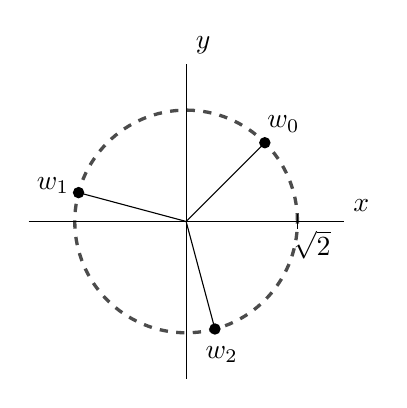
\begin{tikzpicture}
        \draw[color=black!70, very thick, dashed] (0,0) circle (1.414);
        \draw (-2,0) -- (2,0) node[anchor=south west] {$x$};
        \draw (0,-2) -- (0,2) node[anchor=south west] {$y$};
        \draw (1.414,0.1) -- (1.414,-0.1);
        \node at (1.6, -0.3) {$\sqrt{2}$};
        % drawing points
        \filldraw[color=black, very thick] (45:1.414) circle (0.05);
        \draw (0,0) -- (45:1.414);
        \node at (45:1.75) {$w_0$};
        \filldraw[color=black, very thick] (165:1.414) circle (0.05);
        \draw (0,0) -- (165:1.414);
        \node at (165:1.75) {$w_1$};
        \filldraw[color=black, very thick] (285:1.414) circle (0.05);
        \draw (0,0) -- (285:1.414);
        \node at (285:1.75) {$w_2$};
    \end{tikzpicture}
\end{center}

\question Assuming that $|z_3| \ne |z_4|$, show that
\[
  \frac{ \re(z_1+z_2)}{|z_3+z_4|} \le \frac{|z_1| +
    |z_2|}{||z_3|-|z_4||}.
\]
To show the above inequality, we show that the numerator on the RHS is greater than the numerator on the LHS and the denominator on the RHS is less than the denominator on the LHS.
We first show that $\re (z_1 + z_2) \leq |z_1| + |z_2|$.
Consider $\re (z_1 + z_2) = \re (x_1 + iy_1) + (x_2 + iy_2) = \re (x_1 + x_2 + i(y_1 + y_2)) = x_1 + x_2$.
Then $x_1 + x_2 \leq \sqrt{x_1^2} + \sqrt{x_2^2} \leq \sqrt{x_1^2 + y_1^2} + \sqrt{x_2^2 + t_2^2} = |z_1| + |z_2|$.
Then we can show that $|z_3 + z_4| \geq ||z_3| - |z_4||$.
Beginning with $|z_3 + z_4| = |z_3 - -z_4| \geq ||z_3| - |-z_4|| = ||z_3| - |z_4||$.
Since $|z_3| \ne |z_4|$, the denomonitor on the RHS is not 0, so the expression is defined.
Therefore,
\[
  \frac{ \re(z_1+z_2)}{|z_3+z_4|} \le \frac{|z_1| +
    |z_2|}{||z_3|-|z_4||}.
\]

\question Use de Moivre's formula to derive the trigonometric
identities
\begin{align*}
  \cos (3\theta) &= \cos^3 \theta - 3 \cos \theta \, \sin^2 \theta, \\
  \sin (3\theta) &= 3 \cos^2 \theta \, \sin \theta -  \sin^3 \theta.
\end{align*}
We begin with $\exp (i\theta) = \cos \theta + i \sin \theta$.
Then $(\exp (i\theta))^3 = (\cos \theta + i \sin \theta)^3$.
Expanding the RHS,
\begin{align*}
    (\cos \theta + i \sin \theta)^3
    &= \cos ^3 \theta + 3 \cos ^2 \theta (i \sin \theta) + 3 \cos \theta (i \sin \theta)^2 + (i \sin \theta)^3 \\
    &= \cos ^3 \theta + i3 \cos ^2 \theta \sin \theta + i^2 3 \sin ^2 \theta \cos \theta + i^3 \sin ^3 \theta \\
    &= \cos ^3 \theta - 3 \sin ^2 \theta \cos \theta + i(3 \cos ^2 \theta \sin \theta - \sin ^3 \theta)
\end{align*}
Then the LHS is $(\exp (i\theta))^3 = \exp (i3\theta) = \cos (3 \theta) + i \sin (3 \theta)$.
Since the LHS must equal the RHS, the real and imaginary parts of each side must match.
This gives us
\begin{align*}
  \cos (3\theta) &= \cos^3 \theta - 3 \cos \theta \, \sin^2 \theta, \\
  \sin (3\theta) &= 3 \cos^2 \theta \, \sin \theta -  \sin^3 \theta.
\end{align*}

\question In each case, sketch the set of points determined by the
given condition.
\begin{parts}
  \part $|z-2+i| \le 1$ \\
        $|z-2+i| = | z- (2-i)| \leq 1$: \\
        \begin{center}
        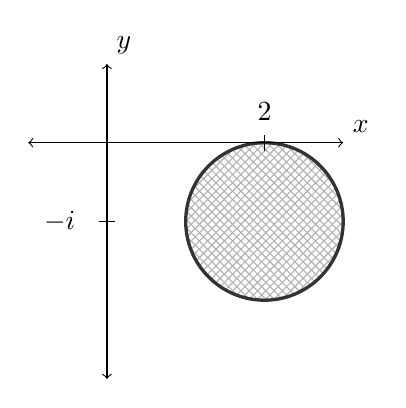
\begin{tikzpicture}
            \draw[color=black!80, very thick, pattern=crosshatch, pattern color=gray!60] (2,-1) circle (1);
            \draw[<->] (-1,0) -- (3,0) node[anchor=south west] {$x$};
            \draw[<->] (0,-3) -- (0,1) node[anchor=south west] {$y$};
            \draw (2,0.1) -- (2,-0.1);
            \node at (2,0.4) {$2$};
            \draw (-0.1,-1) -- (0.1,-1);
            \node at (-0.6,-1) {$-i$};
        \end{tikzpicture}
        \end{center}
  \part $|2z+3| > 4$ \\
          $|2z+3| = | 2(z + 3/2)| = 2 |z - -3/2| > 4 \iff |z - -3/2| > 2$: \\
          \begin{center}
          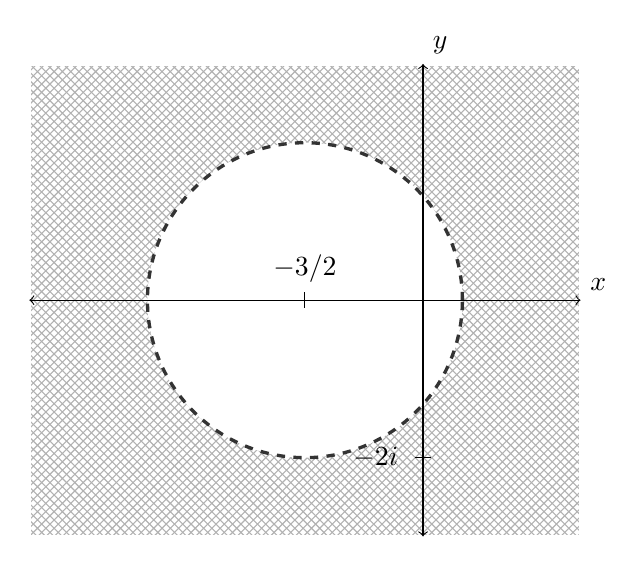
\begin{tikzpicture}
              \draw[color=black!0, very thick, pattern=crosshatch, pattern color=gray!60] (-5,-3) rectangle (2,3);
              \filldraw[color=black!80, fill=white, very thick, dashed] (-1.5,0) circle (2);
              \draw[<->] (-5,0) -- (2,0) node[anchor=south west] {$x$};
              \draw[<->] (0,-3) -- (0,3) node[anchor=south west] {$y$};
              \draw (-1.5,0.1) -- (-1.5,-0.1);
              \node at (-1.5,0.4) {$-3/2$};
              \draw (-0.1,-2) -- (0.1,-2);
              \node at (-0.6,-2) {$-2i$};
          \end{tikzpicture}
          \end{center}
  \part $|z-1| < |z+i|$ \\
        $|z-1| < |z+i| \iff |x-1 + iy| < |x +i(y+1)| \iff
        \sqrt{(x-1)^2 + y^2} < \sqrt{x^2 + (y+1)} \iff
        x^2 -2x + 1 + y^2 < x^2 + y^2 + 1 \iff
        -2x < 2y \iff y > -x$
        \begin{center}
        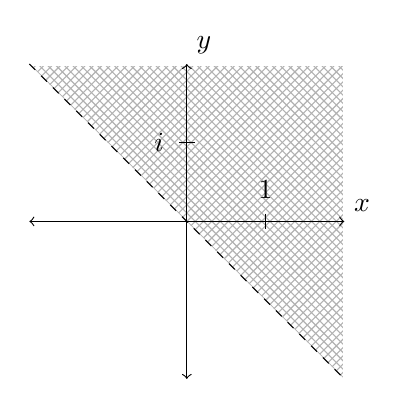
\begin{tikzpicture}[domain=-2:2]
            \draw[color=black!0, very thick, pattern=crosshatch, pattern color=gray!60] (-2,2) -- (2,2) --(2,-2);
            \draw[<->] (-2,0) -- (2,0) node[anchor=south west] {$x$};
            \draw[<->] (0,-2) -- (0,2) node[anchor=south west] {$y$};
            \draw (1,0.1) -- (1,-0.1);
            \node at (1,0.4) {$1$};
            \draw (-0.1,1) -- (0.1,1);
            \node at (-0.35,1) {$i$};
            \draw[dashed] plot (\x,-\x);
        \end{tikzpicture}
        \end{center}
  \part $(\re z) (\im z) > 1$ \\
        $(\re z) (\im z) > 1 \iff xy > 1 $
        \begin{center}
        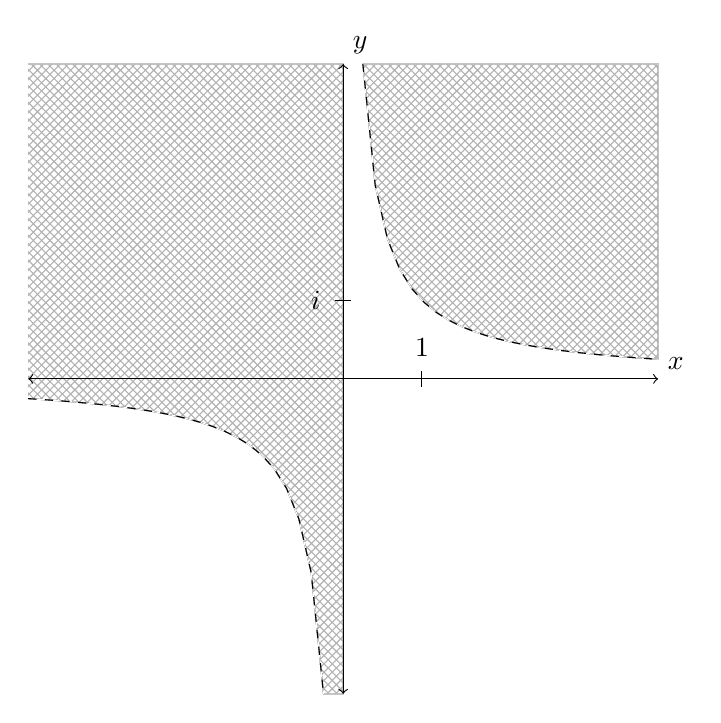
\begin{tikzpicture}
            \draw[domain=-4:-0.25, pattern=crosshatch, pattern color=gray!60] plot (\x,1/\x) -- (0,-4) -- (0,4) -- (-4,4);
            \draw[domain=0.25:4, pattern=crosshatch, pattern color=gray!60] plot (\x,1/\x) -- (4,4) -- (0.25,4);
            \draw[color=white, domain=-4:-0.25] plot (\x,1/\x) -- (0,-4) -- (0,4) -- (-4,4);
            \draw[color=white, domain=0.25:4] plot (\x,1/\x) -- (4,4) -- (0.25,4);
            \draw[<->] (-4,0) -- (4,0) node[anchor=south west] {$x$};
            \draw[<->] (0,-4) -- (0,4) node[anchor=south west] {$y$};
            \draw (1,0.1) -- (1,-0.1);
            \node at (1,0.4) {$1$};
            \draw (-0.1,1) -- (0.1,1);
            \node at (-0.35,1) {$i$};
            \draw[dashed, domain=-4:-0.25] plot (\x,1/\x);
            \draw[dashed, domain=0.25:4] plot (\x,1/\x);
        \end{tikzpicture}
        \end{center}
  \part $0 < \arg z < \pi/4$
      \begin{center}
      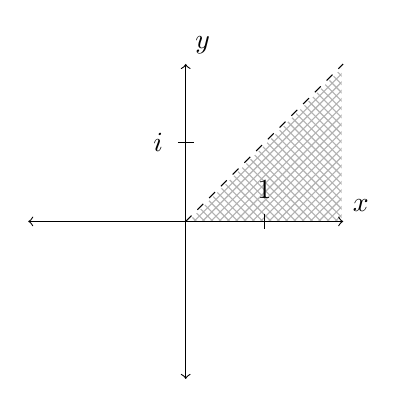
\begin{tikzpicture}[domain=0:2]
          \draw[color=black!0, very thick, pattern=crosshatch, pattern color=gray!60] (0,0) -- (2,2) -- (2,0);
          \draw[<->] (-2,0) -- (2,0) node[anchor=south west] {$x$};
          \draw[<->] (0,-2) -- (0,2) node[anchor=south west] {$y$};
          \draw (1,0.1) -- (1,-0.1);
          \node at (1,0.4) {$1$};
          \draw (-0.1,1) -- (0.1,1);
          \node at (-0.35,1) {$i$};
          \draw[dashed] plot (\x,\x);
      \end{tikzpicture}
      \end{center}
\end{parts}
\end{questions}
\end{document}
